Many areas of science are building unprecedented high resolution and high rate instruments, with ever-increasing granularity and channel count. Consequently,  future data sets  (e.g., from experiments at the RHIC and LHC particle accelerators) will exceed today's standards by an order of magnitude and more (e.g., CMS@LHC tape usage will grow from 250 PB in 2018 to 3000 PB in 2028). Furthermore, the expected data rates have corresponding implications for  Data Acquisition (DAQ) systems, which would have to be more complex, for data transfer systems, which would need increased bandwidth, and for the long term mass storage systems (which would need expanded capacity). In addition, the complexity of big-data analyses increased non-linearly as a function of the data size itself. At present, the scientific community is trying to reduce experimental data volumes using two parallel approaches: by developing highly selective event selection systems (\eg real-time event selection or `online triggering'), and by compressing data, through high-performance data compression algorithms. Triggering is limited by the performance (\ie, efficiency, speed) of trigger algorithms, which rely on a fast, but incomplete, reconstruction of data and hence provide a potentially biased selection. While this approach largely preserves data fidelity, it is too resource-demanding in particular in light of ever-increasing data rates. Similar challenges arise outside of science, e.g., in an industrial context with the rise of the Industrial Internet of Things (IIoT). While in this proposal we will take two nuclear physics experiemns as example the method/approach/algorithm we are going to describe is general and may be applied to different science fields and applications. 

 Most compression algorithms used in particle physics experiments are lossless, achieving only a limited compression while preserving all information, signal or noise, in the data.  Higher compression levels may be achieved using lossy compression techniques, that not only reformat the data to reduce its size but also strip out some information. However, the tuning of the lossy algorithms needs to be tailored to the use-case, and carefully validated against the analysis physics goal of the dataset collected. This traditional approach is extremely expensive in terms of workforce, with generally slow turnaround cycles. The selection and tuning of the lossy compression algorithm are also particularly complex as the compressed information should be general enough to accommodate future and not yet foreseen analyses. A data event recorded by a detector (\eg, sPHENIX, CMS) typically comprises a collection of RAW data produced by the sub-detectors composing the experiment. In general, each of the sub-detectors has a unique data format, so to achieve the highest compression factor, each sub-detector data needs to be treated independently with specific compression algorithms and/or tuning. The RAW data tier is also only the first tier in the data analysis process, is further processed to create general Analysis Object Data (AOD), and then processed again to create smaller AOD versions (\eg, nano-AOD), targeted to specific data analysis. This multi-tier approach is essential to minimize the need for data reprocessing, but it has a negative effect on the total amount of storage space. To achieve efficient data reduction, each data tier should be compressed with a dedicated compression algorithm specifically tuned for the purpose, as shown in Fig.~\ref{fig:concept} (left). But, the high dimensionality of any general lossy compression algorithm renders a simple recursive approach (for tuning) infeasible. 

We propose a different approach: to create a Machine Learning (ML) framework, which includes image recognition techniques, trained on data and/or simulations, able to identify and tune the most efficient algorithms, with supervisory ML algorithms ensuring the required data fidelity. The framework, using a Deep Neural Network (DNN) and the recently developed Generative Adversarial Networks (GAN), will be built to achieve two goals: i) to create the next generation online trigger algorithms, in which real data will be seen as an image in which physics objects can be identified without the needs of their full reconstruction, improving on the speed and accuracy of the selection; ii) to create the ultimate step-by-step data compression algorithms, in which the framework will learn the requirements of the final physics object (e.g., thresholds, biases, etc.) and will select an optimal set of algorithms for the task, as well as their settings, during each step of data processing. 

Figure \ref{fig:concept} (left) shows the interaction between the data flow and the proposed ML framework. First, the ML optimizes the online triggering. Then, the ML Optimizer collects information from the data-tiers and  physics analysis objects and learns the peculiarity of the various components. The ML Optimizer selects the most appropriate lossy compression algorithm for each data-tier from a library and computes the best algorithm settings. The full workflow including the compression of data tiers is then executed, and the cycle is repeated up to the definition of the algorithms and parameters to be used in the production system. Continuous tuning on the fly, directly in the production system, is also considered.   

\begin{figure}[!ht]
    \vspace{-0.4cm}
    \begin{center}
    \scalebox{1}[1]{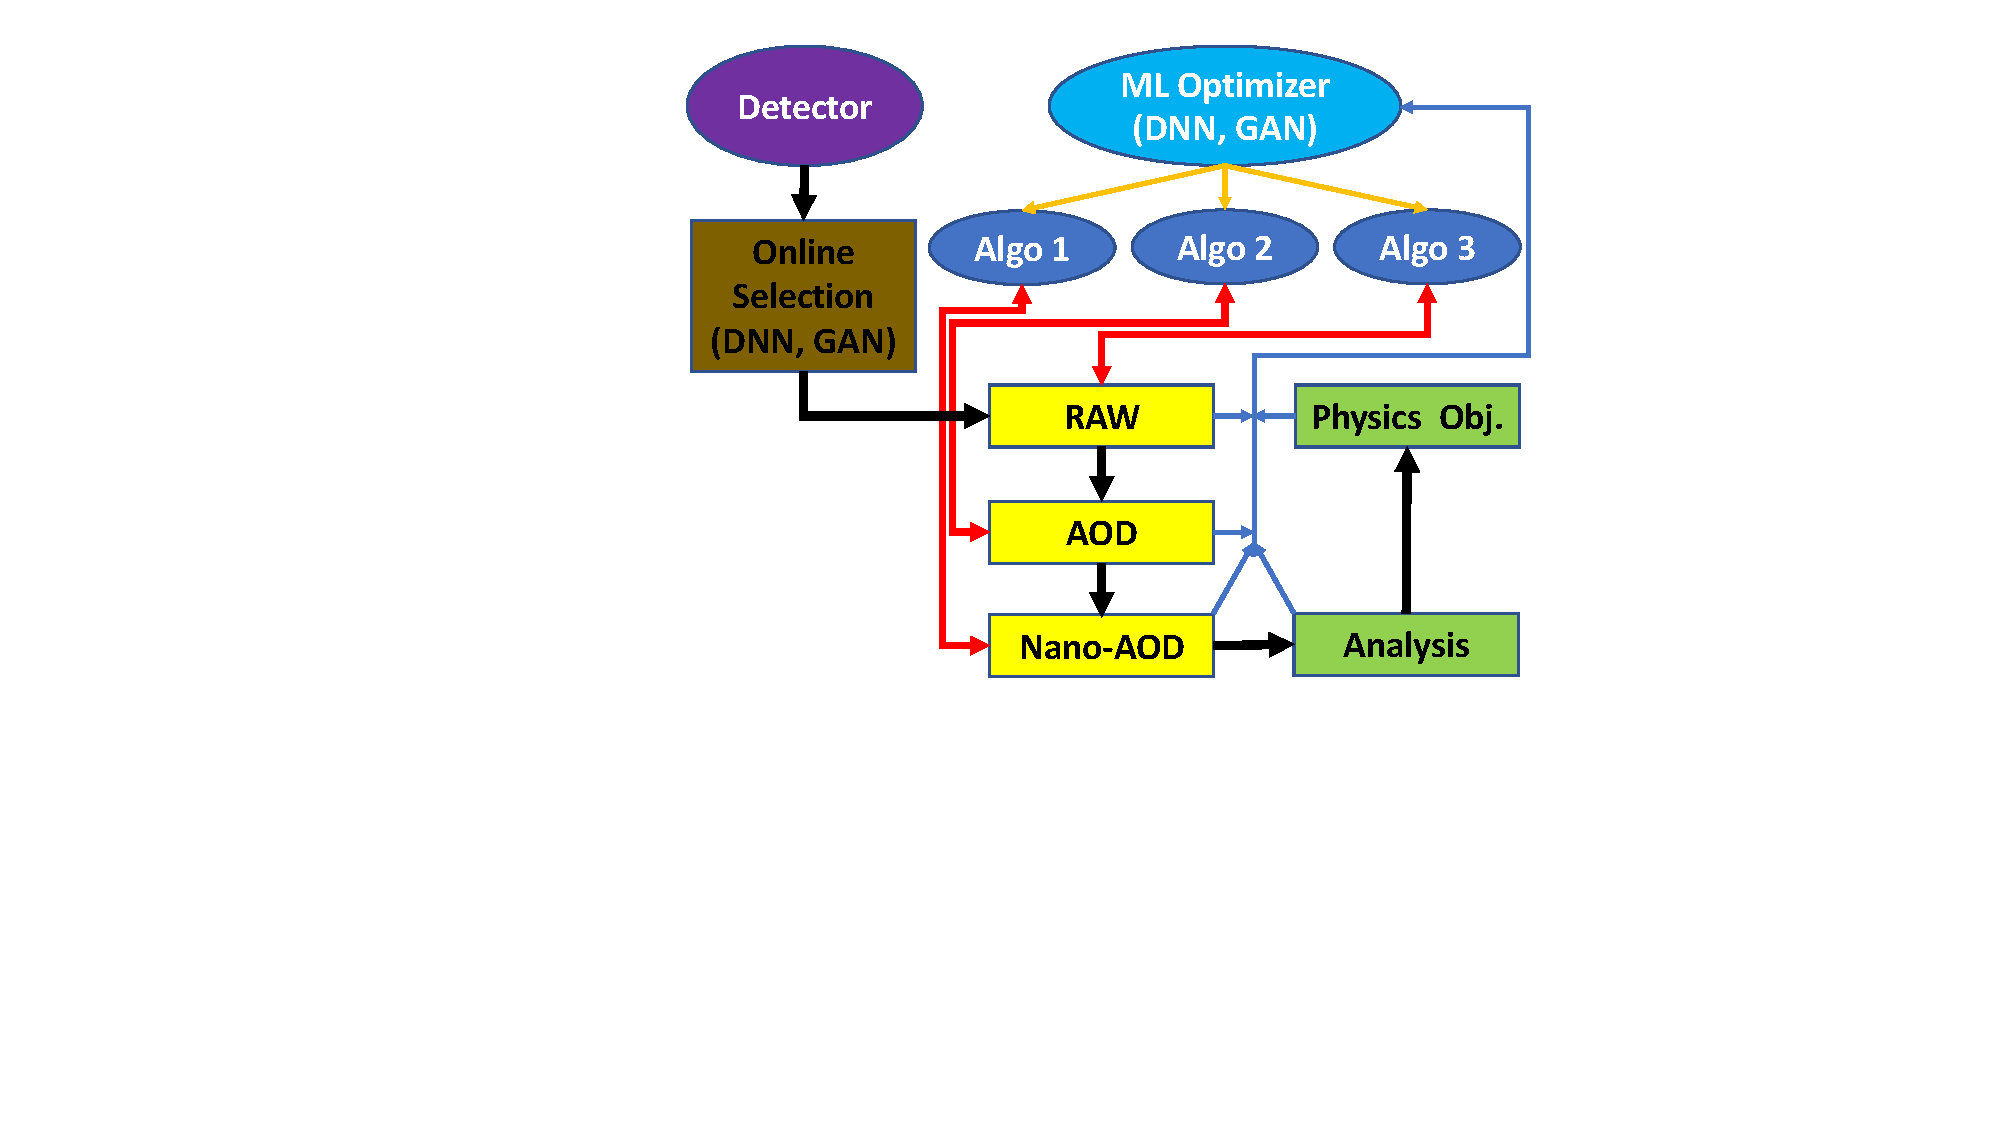
\includegraphics[width=.34\textwidth]{HI_Compress/figure/CompSchemaV4.pdf}}
    %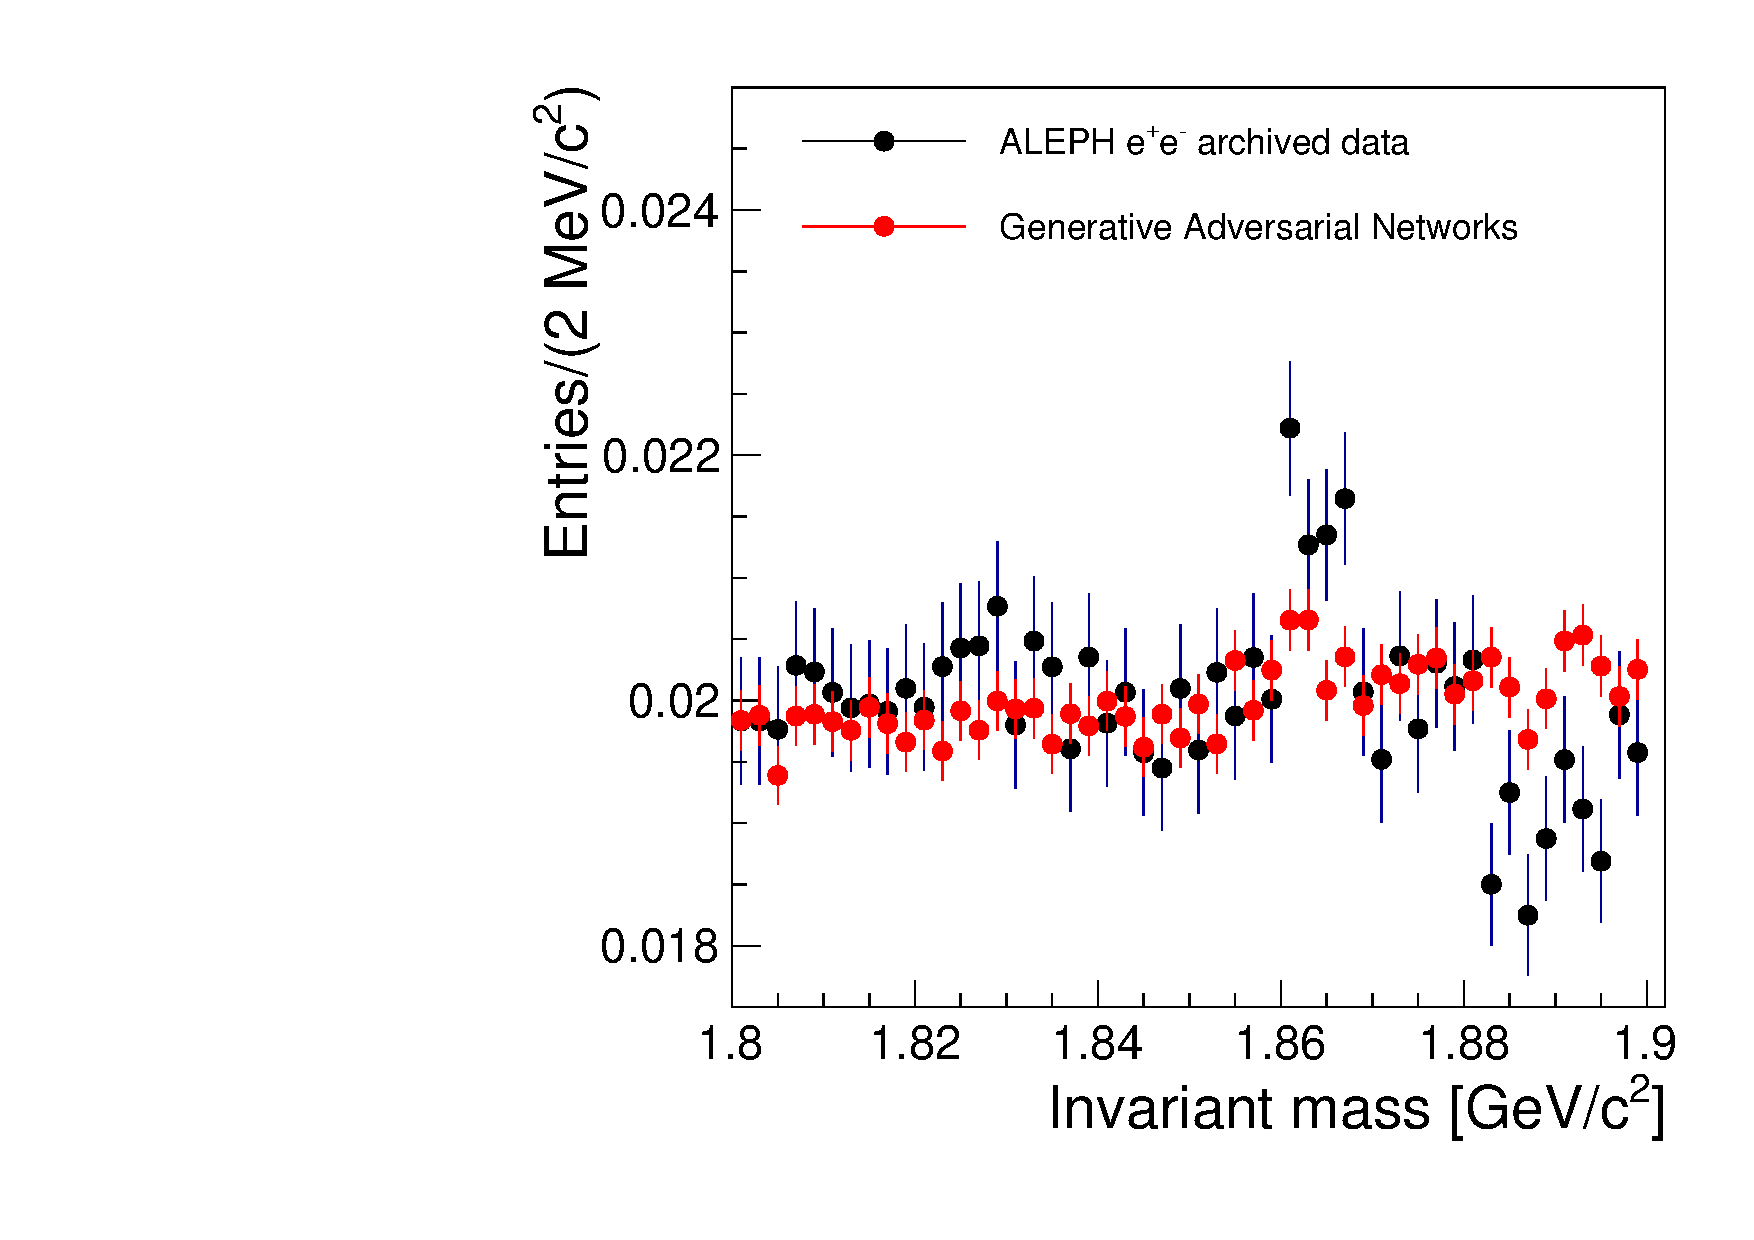
\includegraphics[width=.25\textwidth,keepaspectratio]{outputFig}
    \hspace{0.03\textwidth}
    %\includegraphics[width=.25\textwidth,keepaspectratio]{}
    \scalebox{1}[1]{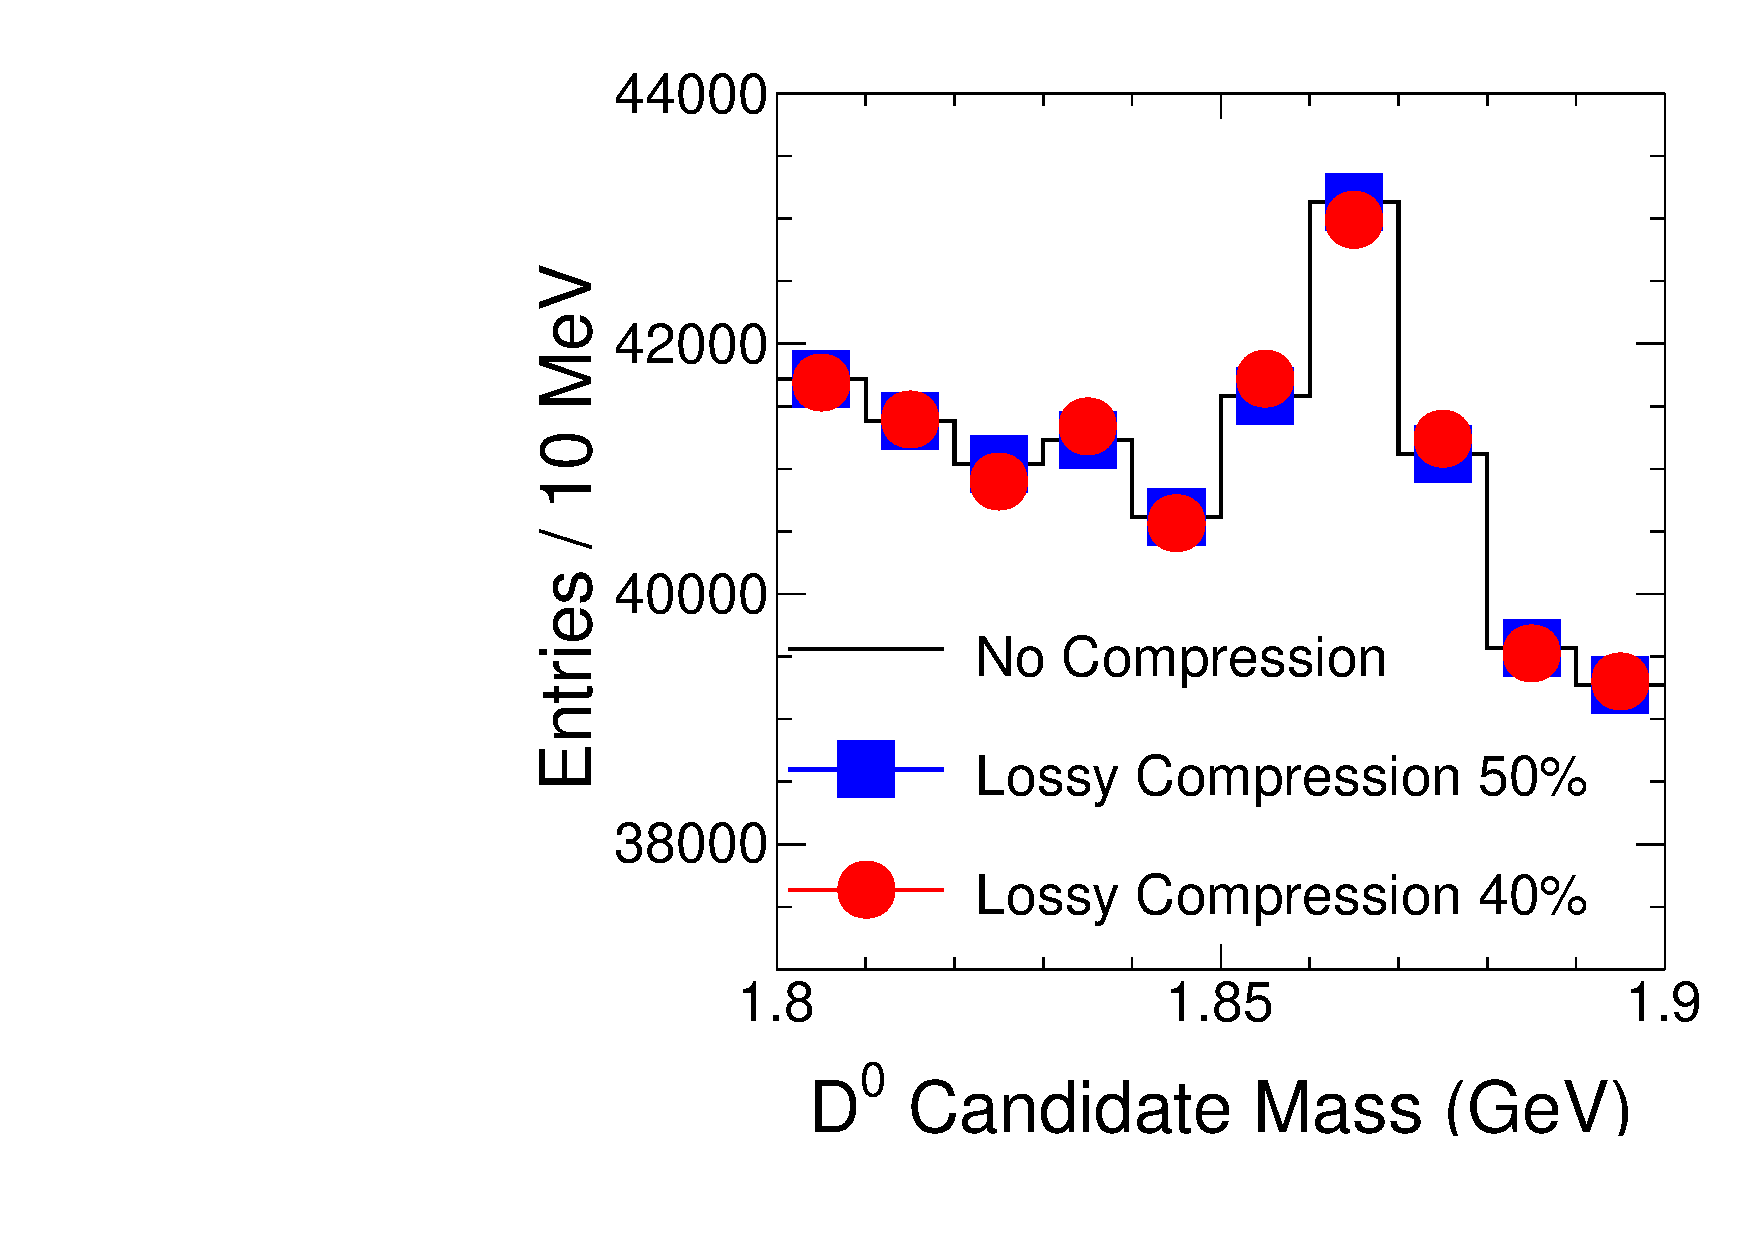
\includegraphics[width=.28\textwidth,keepaspectratio]{HI_Compress/figure/aleph/Performance_v6.pdf}}
     \scalebox{1}[1]{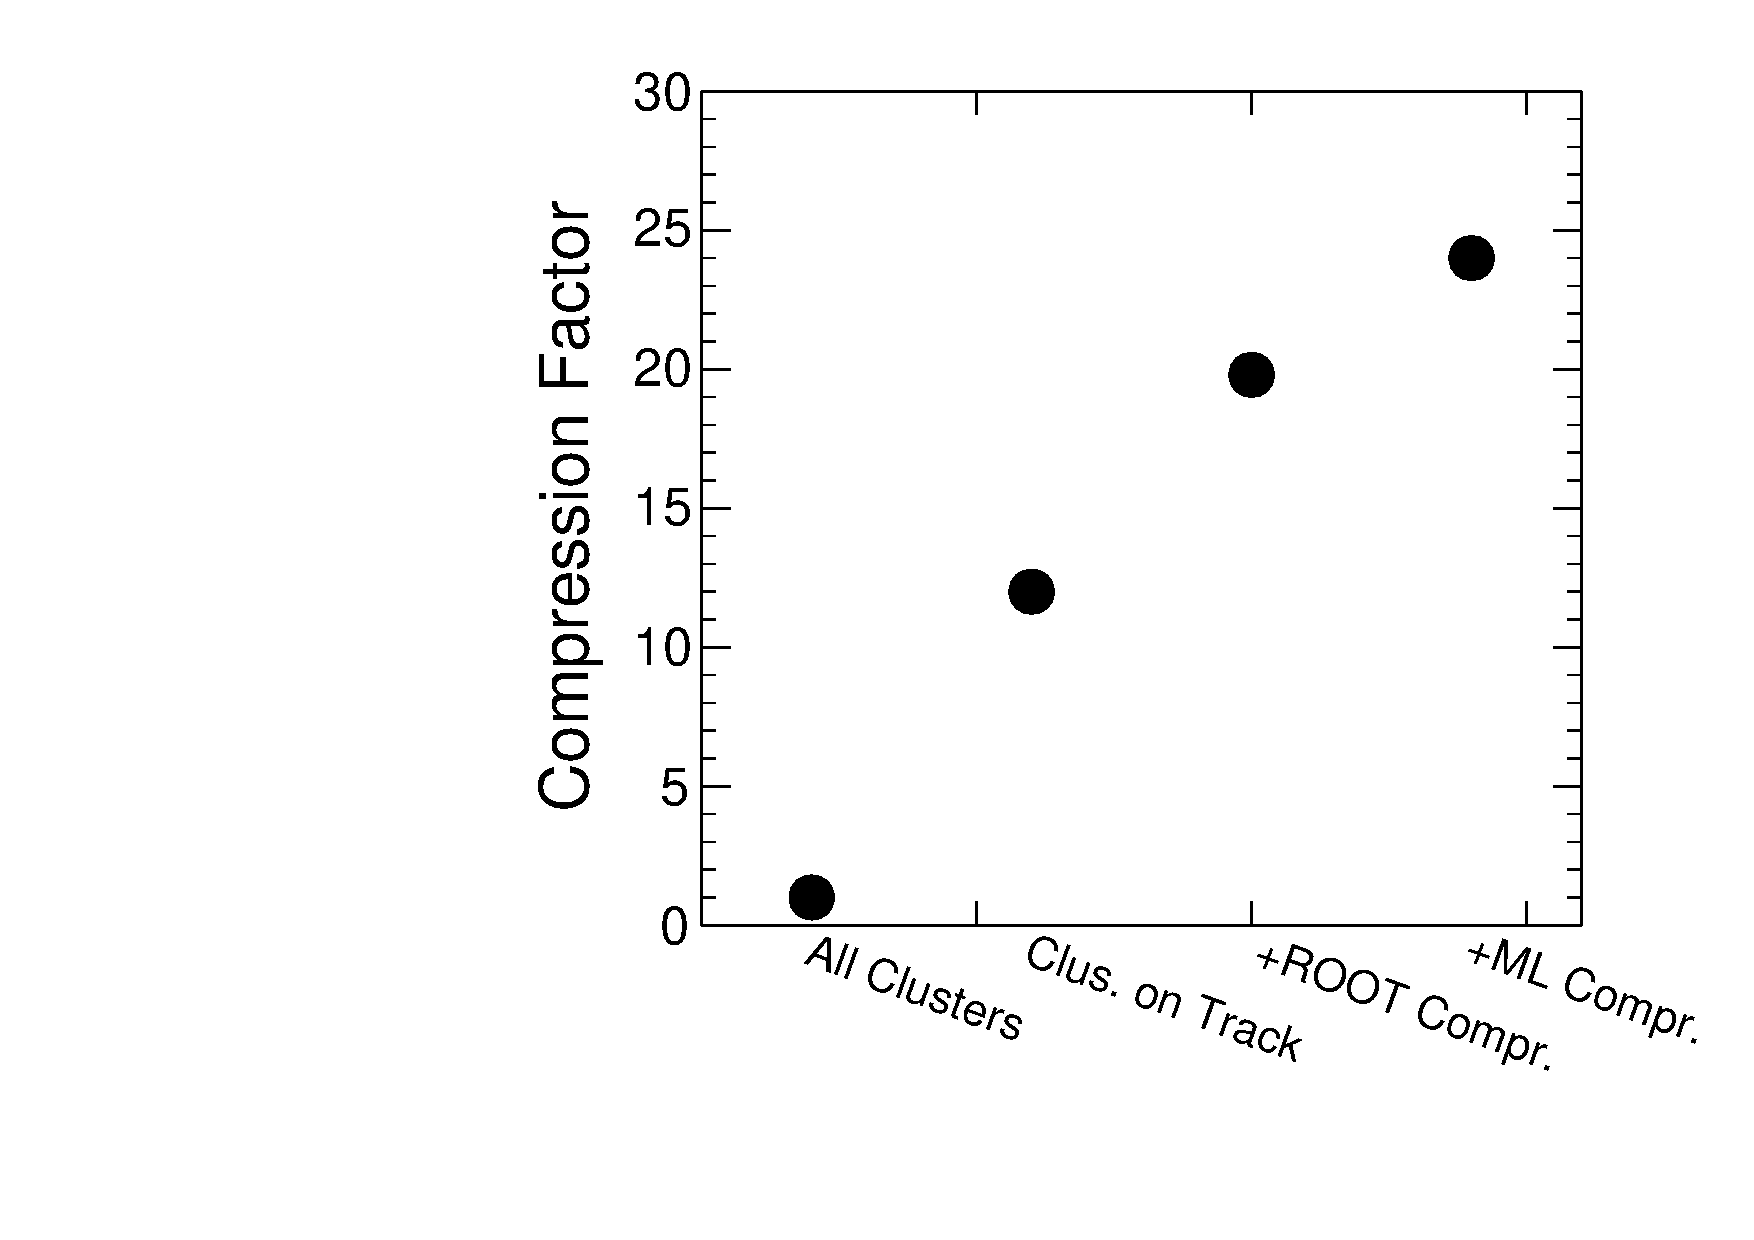
\includegraphics[width=.295\textwidth,keepaspectratio]{HI_Compress/figure/sphenix_comp_v3.pdf}}
    \vspace{-0.5cm}
    \caption{Left: Flowchart showing data interactions withe ML framework. Center: $D^0$ meson mass spectra with two compression algorithm tunes. Right: Compression factor achieved for sPHENIX TPC cluster data.}
    \label{fig:concept}
    \end{center}
\end{figure}
%s
\vspace{-0.8cm}
We have already selected a candidate lossy algorithm that is being studied in  IIoT applications. These share several fundamental requisites with high-energy experimental physics: having to process live streaming data, in cost-effective ways. The proposed data-reduction algorithm will support in-stream processing of data by using the Unsupervised Incremental Binning (UIB) technique, which is based on the online agglomerative clustering method. UIB groups individual values into a small but sufficient maximum number of bins (default maximum is 65,536 bins) with each bin recording observed statistical properties. Upon a newly observed value, UIB creates a new bin; when the total number of created bins exceeds the default maximum quantity, the two nearest bins are identified by a distance-comparison procedure and then merged. Similar values will be merged as a cluster with outliers being accurately approximated, as opposed to existing clustering algorithms that do not deal with outliers, and which can not easily support in-stream processing. Furthermore, with such a high maximum count set, bins can be represented by 16-bit short integers instead of the original 32-bit floating-point values, and hence data volume can be reduced by at least a factor of two. The complexity of the proposed algorithm will be $O(\log(k))$ for processing a newly observed value, where $k$ stands for the number of maximum bins in the algorithm. The target data size is tune-able based on this lossy compression algorithm. 

The proposed algorithm has been tested on archived RAW data collected by the ALEPH collaboration at LEP. Figure \ref{fig:concept} (middle) shows the comparison of the $D^0$ candidate mass calculated with and without compressing the RAW data with the UIB algorithm, using two settings corresponding to different compression levels. %Moreover, preliminary studies using the UIB algorithm for the two main data producers of two flagship detectors in particle and nuclear physics, CMS@LHC and sPHENIX@RHIC, gave a size reduction of roughly 40\%-50\% without affecting the physics performance.  
Figure \ref{fig:concept} (right) shows the compression factor achieved for cluster data of the sPHENIX TPC. Selecting clusters on reconstructed tracks reduces the data volume from out-of-time pileup events and yields a compression factor of $\approx 12$. Adding an ML guided algorithm to reduce the cluster information to a minimum number of bits to store the position information increases the compression factor to $\approx 24$, compared to a benchmark value of $\approx 20$ achieved with the ROOT software framework. More lossy algorithms will be developed and explored during the project.

In summary, the proposal aims to conduct foundational research to develop reliable and efficient ML tools and new computational technologies to address one of the most challenging problems in many areas of research: the size of exascale datasets collected by high-resolution giga-channel instruments. While in this proposal we have been focusing on the nuclear physics scientific domain, the algorithm mentioned is general enough to be used for any application involving big datasets/big bandwidth applications.  At the time of writing the algorithm is being applied/evaluated in three fields like High-Energy Physics, Nuclear Physics and industrial processes (e.g. Silicon Test data compression). It is worth mentioning that also the application in the various domains is general allowing the processing of eterogenous data types (e.g. RAW data, clusters, industrial monitoring data, etc). 
\clearpage
